\chapter{Shape Sensitivity Analysis using Immersed Boundary Method}
In this chapter we apply the continuum sensitivity analysis to the CFD simulations conducted using the Immersed Boundary (IB) method. In this chapter the focus is on calculating the sensitivity of flow variables such as pressure and velocity to the design variable that controls the shape of the boundary, i.e. radius of a cylinder, camber of an airfoil. The boundary of the solid domain is represented using an analytical function. However, as will be shown in the following chapters this is not a required for this method. In this chapter the modifications on the IB approach to make it suitable for continuum sensitivity formulation is discussed. To the best of the author's knowledge, this is the first time that sensitivity analysis is done for CFD simulations based the continuum IB formulation.
% ======================================================================================
\section{Sensitivity Problem Formulation}
In contrast to traditional body conformal methods, in IB approach the solid boundaries are represented by modifying the governing equation near the boundaries. In the case of continuum IB method, this is done by adding the appropriate force term to the cells adjacent to the immersed boundary. The value of these forces are calculated either using a feedback forcing \cite{goldstein1993modeling} or a penalization function \cite{arquis1984conditions}. The Navier-Stokes (NS) equations are written as shown in Equation \eqref{eq:C4_NS}.

\begin{equation}\label{eq:C4_NS}
	\frac{\partial \mathbf{u}}{\partial t} + \mathbf{u} \cdot \nabla \mathbf{u} = 
	-\frac{\nabla P}{\rho} + \mu \nabla^2 \mathbf{u} + \mathbf{f}
\end{equation}

where $\mathbf{u}$ is the velocity vector, $P$ is pressure, $\mu$ is the kinematic viscosity ($\mu / \rho$), $\rho$ is density, and $\mathbf{f}$ is the forcing term. The NS equations are solved on a Eulerian grid that is fixed in space and the IB is defined on a separate Lagrangian grid that can move. This is shown Figure \ref{fig:C4_lagrangianAndEulerianDomain}.

\begin{figure}[H]
	\centering
	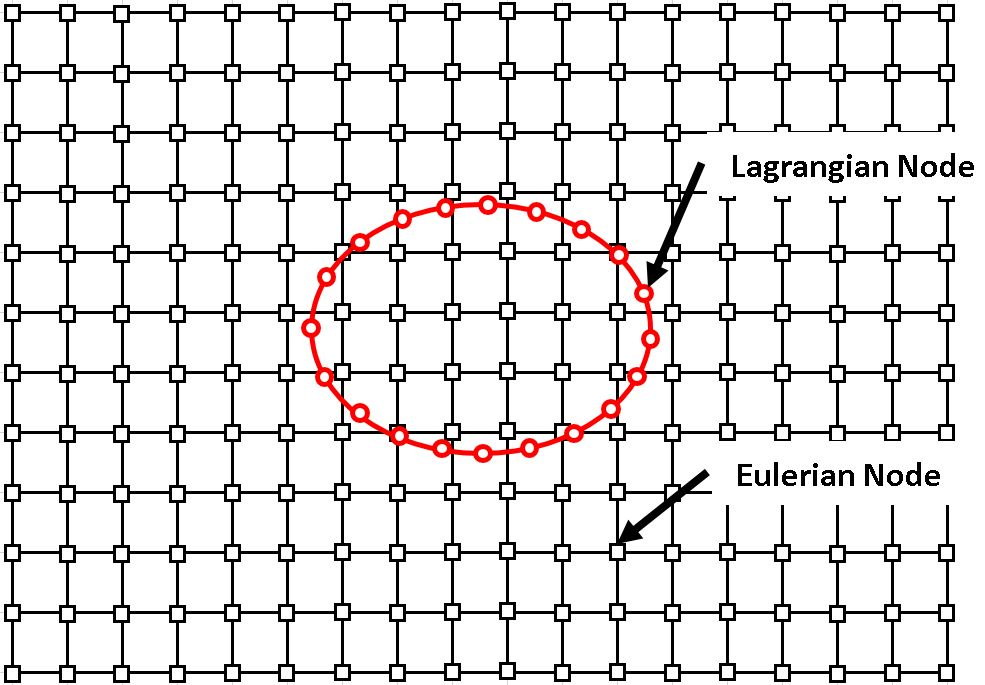
\includegraphics[width=7.00cm]{Chapter_4/figure/lagrangian_and_eulerian_nodes.jpg}
	\caption{Eulerian and Lagrangian nodes for representing the fluid and solid domain. The Eulerian and Lagrangian nodes are represented by black squares and red circles.}
	\label{fig:C4_lagrangianAndEulerianDomain}
\end{figure}

The forcing function in the penalization method is calculated at the \emph{Eulerian} nodes and is applied to computational nodes inside the solid boundary using a step function as shown in Equation \eqref{eq:C4_penalizationForcingFunction}.

\begin{equation}\label{eq:C4_penalizationForcingFunction}
	\mathbf{f} = -\mathcal{S}(\mathcal{X}(b)) \kappa \mathbf{u}
\end{equation}

where $\mathcal{S}$ is the step function, $\mathcal{X}$ defines the relative location of locations inside the domain with respect to the IB boundary, $\kappa$ is the penalization parameter, and $\mathbf{u}$ is the fluid velocity. Using this forcing function, the governing equation \eqref{eq:C4_NS} is rewritten as shown in Equation \eqref{eq:C4_NSwithPenalization}

\begin{equation}\label{eq:C4_NSwithPenalization}
	\frac{\partial \mathbf{u}}{\partial t} + \mathbf{u} \cdot \nabla \mathbf{u} = 
	-\frac{\nabla P}{\rho} + \mu \nabla^2 \mathbf{u} -\mathcal{S}(\mathcal{X}(b)) \kappa \mathbf{u}
\end{equation}

As mentioned in Chapter \ref{ch:sensitivityAnalysis}, to derive the continuum sensitivity formulation the governing equation of \eqref{eq:C4_NSwithPenalization} is differentiated with respect to the design variable, $b$. The step function $\mathcal{S}$ derivative is Dirac delta function with is singular and cannot be used to solving the governing equations in a numerical framework. Therefore a regularized Heaviside function, $\mathcal{H}$ will be employed instead of the step function for penalizing the governing equation. The effect of this function of the simulation results and sensitivity formulation will be discussed in the following sections.

In the virtual boundary method, the forcing function is calculated at the \emph{Lagrangian} nodes using Equation \eqref{eq:C3_feedbackForcingFunction}.

\begin{equation}\label{eq:C3_feedbackForcingFunction}
	\mathbf{f}(\mathbf{X}, t) = 
	\alpha \int_0^t \left[ \mathbf{u}(\mathbf{X}, \tau) - \mathbf{V}(\mathbf{X}, \tau) \right] d\tau + 
	\beta \left[ \mathbf{u}(\mathbf{X}, \tau) - \mathbf{V}(\mathbf{X}, \tau) \right]
\end{equation}

where $\mathbf{u}(\mathbf{X}, t)$ is the fluid's velocity at the Lagrangian points $\mathbf{X}$ and $\mathbf{V}(\mathbf{X}, t)$ is the desired velocity at the Lagrangian point. For the no-slip boundary condition at the solid boundary, the desired velocity $\mathbf{V}(\mathbf{X}, t)$ is zero at each of the Lagrangian points. The Eulerian nodes where the fluid's governing equation is solved does not necessary coincide with the Lagrangian points. Moreover, the forcing functions that are evaluated at the Lagrangian nodes need to tranfered to the Eulerian nodes where the governing equations for the fluid is solved. As mentioned in Chapter \ref{ch:immersedBoundary}, different mapping functions are used for transferring data between the Lagrangian and Eulerian nodes. However, none of these functions are continuously differentiable as required for the continuum sensitivity analysis. To address this issue a regularized delta function is introduced.

\subsection{Regularized Heaviside/Delta Function}
The regularized Heaviside function is a step function that is smoothed so that its derivative can be calculated numerically. The regularized Heaviside function is also known as sigmoid function in mathematics and is characterized as a real-valued and differentiable, having either a non-negative or non-positive first derivative. There are a pair of horizontal asymptotes as $x \rightarrow \pm \infty$. An example of Heaviside function is shown in Figure \ref{fig:C4_heavisideFunctionExample}.

\begin{figure}[H]
	\centering
	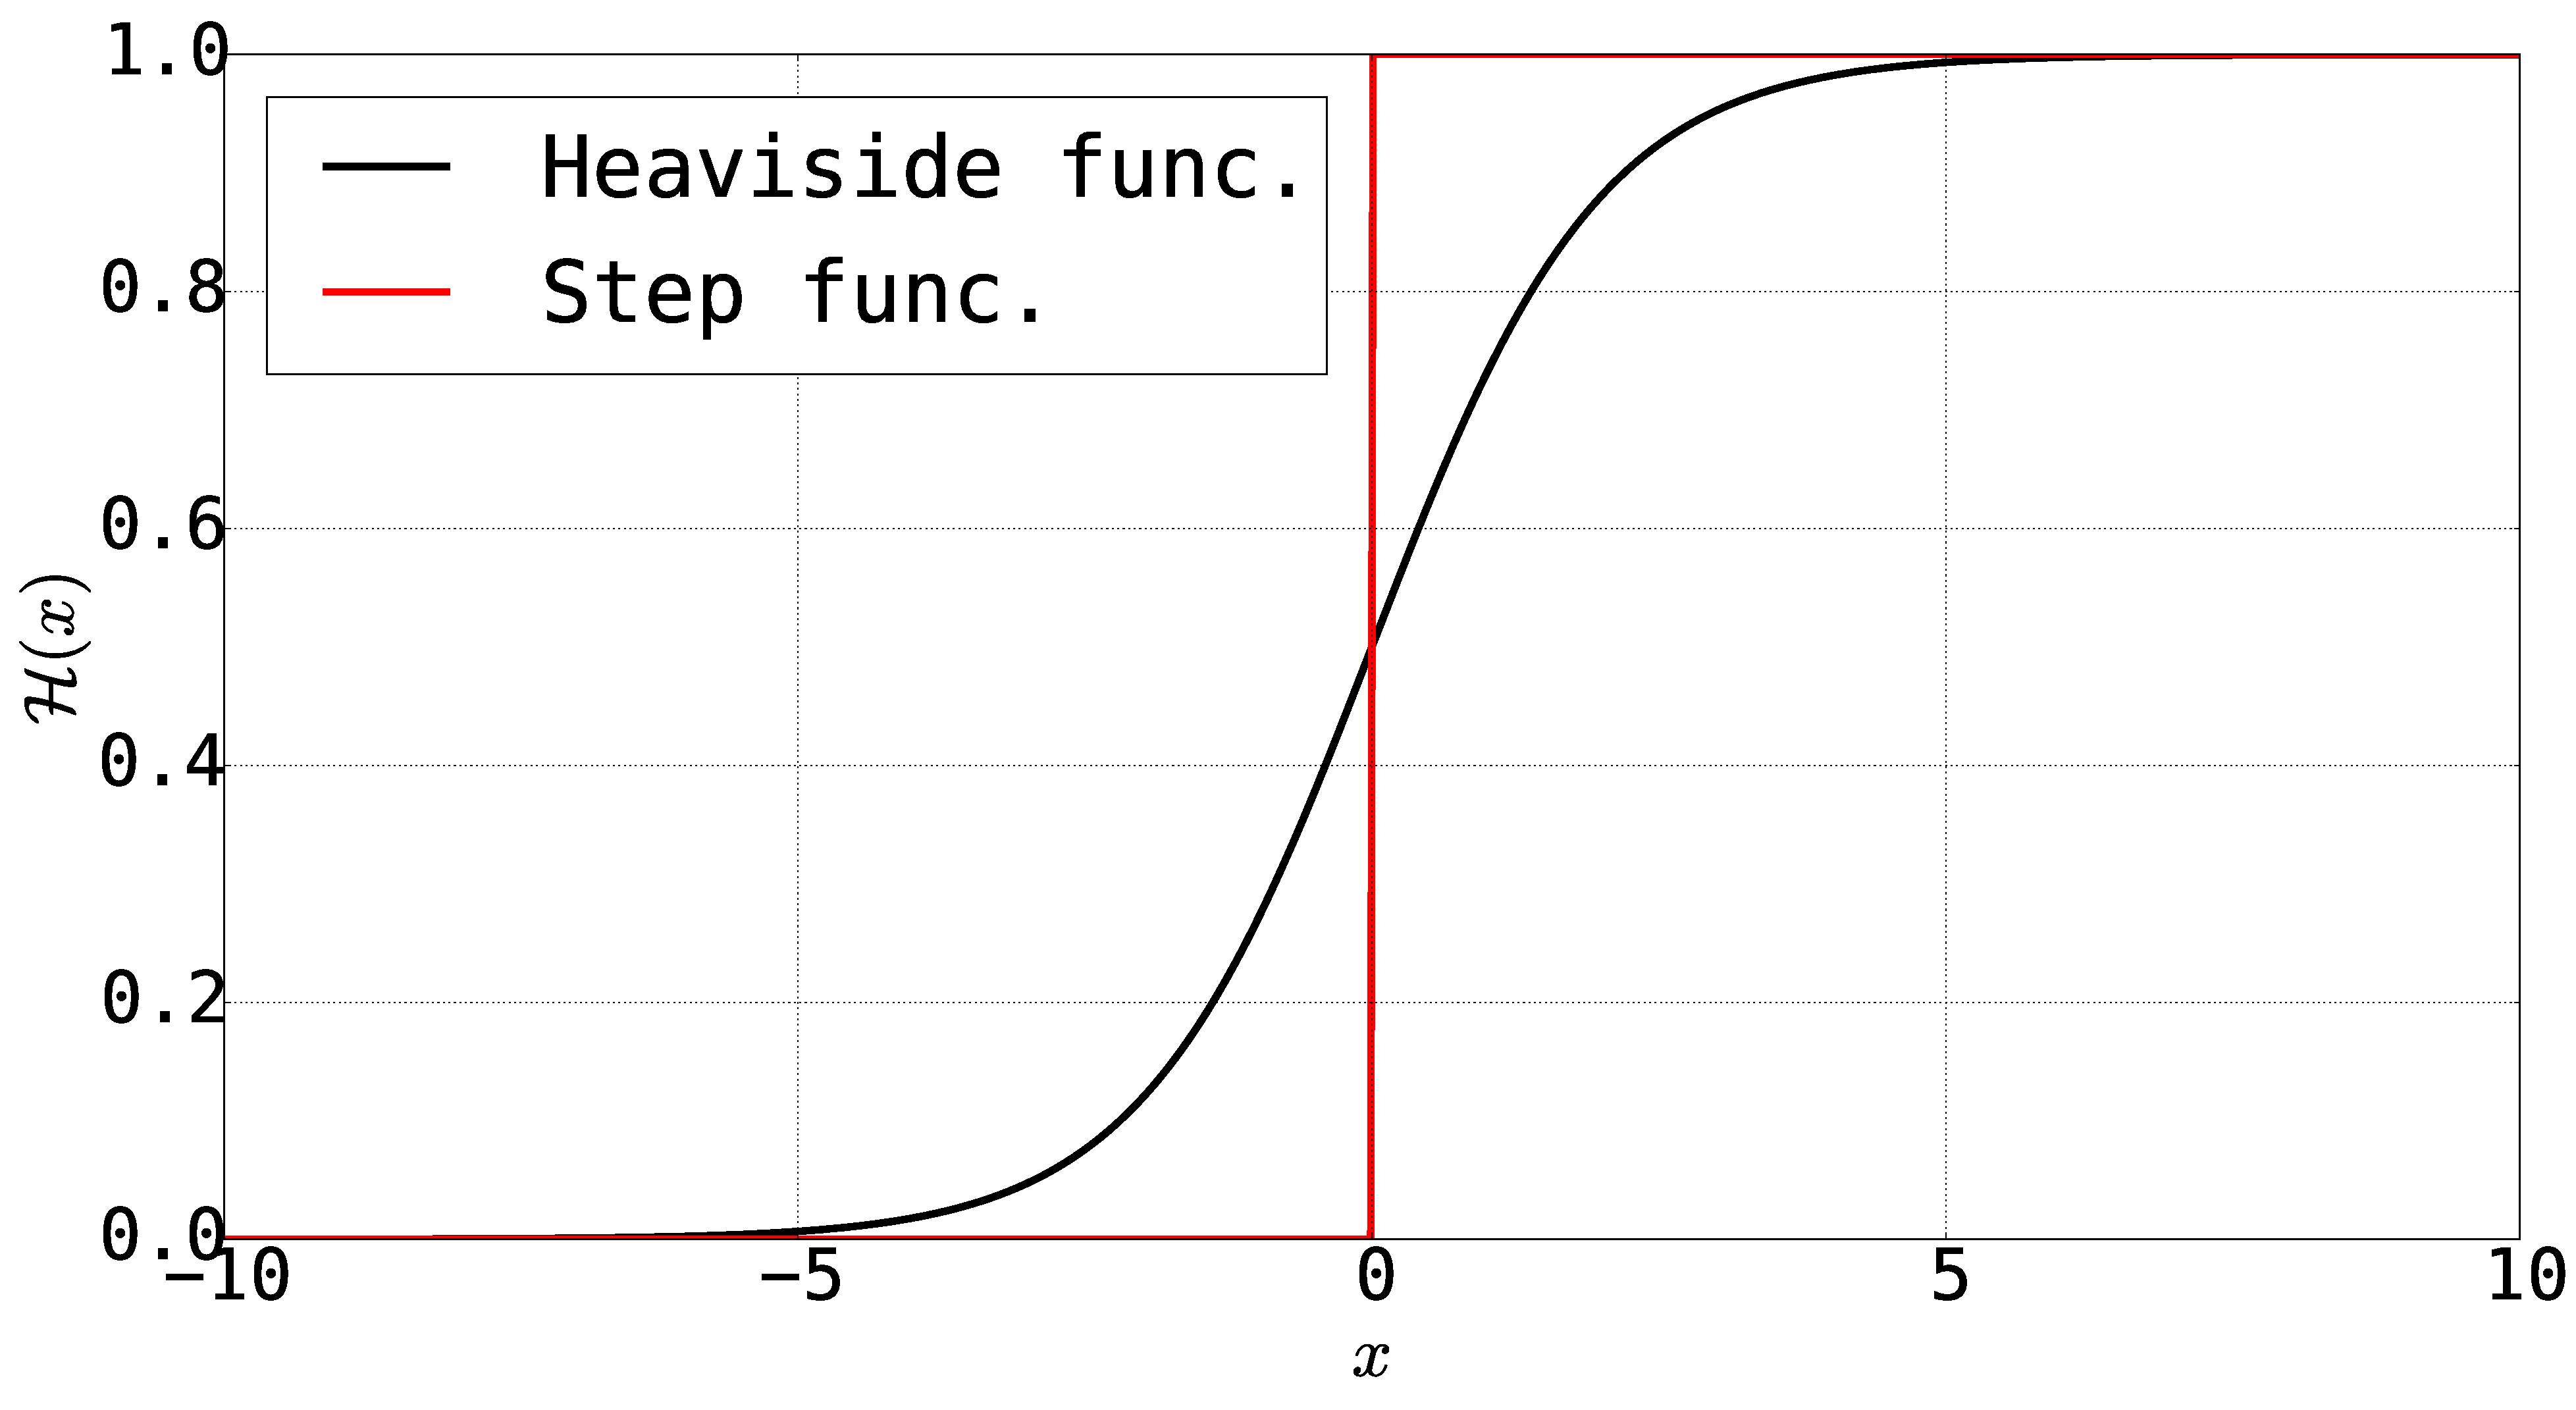
\includegraphics[width=10.00cm]{Chapter_4/figure/heaviside_function_example.eps}
	\caption{Regularized Heaviside function, $\mathcal{H}(x) = 1 / (1 + e^{-x})$.}
	\label{fig:C4_heavisideFunctionExample}
\end{figure}

The regularized Heaviside function is used instead of the step function to penalized the governing equation.

\subsection{Direct Method}

\subsection{Adjoint Method}

\section{Shape Sensitivity Analysis for 1D problem}

\section{Shape Sensitivity of Flow over a Cylinder}

\section{Shape Sensitivity of Flow through a Nozzle}

\section{Summary}
